\chapter[Capítulo 3. Background en algoritmos de árboles de decisión]{Background en algoritmos de árboles de decisión}

\section{Fundamentos de árboles de decisión}

 Los \textbf{árboles de decisión} \cite{ref3} son un tipo de algoritmos de aprendizaje supervisado (tanto para clasificación como para regresión) utilizado en diversos ámbitos como la inteligencia artificial, las finanzas, el marketing, etc. \\ Dado un conjunto de datos se fabrican diagramas de construcciones lógicas en forma de ramificaciones de árboles, muy similares a los sistemas de predicción basados en reglas, que sirven para representar y categorizar una serie de condiciones que ocurren de forma sucesiva, para la resolución de un problema.
 
 Adentrándonos en los aspectos más técnicos de este tipo de modelos de predicción, cabe destacar que las variables de entrada y de salida pueden ser tanto categóricas como continuas y que divide el espacio de los predictores (variables independientes) en regiones distintas y no superpuestas, tal como veremos en la siguiente figura.
 
 \begin{figure}[H]
 	\centering
 	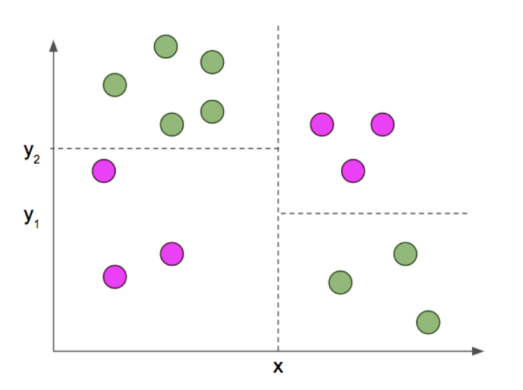
\includegraphics[width=0.7\textwidth]{imagenes/ejemploArboles} 
 	\caption{Ejemplo de árbol de decisión \cite{ref4}}
 \end{figure}
 
 Estas divisiones se realizan creando sobre la población (el conjunto de datos) subconjuntos lo más homogéneos posible entre las muestras que componen un grupo y lo más heterogéneo posible entre los distintos subconjuntos.\\
 Para la efectuación de esta separación, el algoritmo se basa en las variables de entrada más significativas, es decir, las que mejor separan las muestras.
 
 A continuación podemos observar las diferentes partes de un árbol de decisión.
 
  \begin{figure}[H]
 	\centering
 	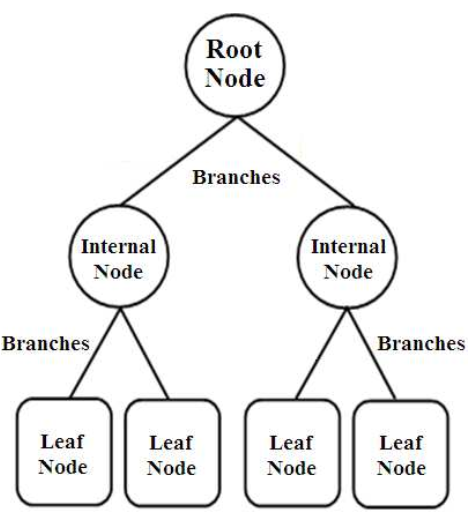
\includegraphics[width=0.5\textwidth]{imagenes/ejemploArbol} 
 	\caption{Partes de un árbol de decisión \cite{ref5}}
 \end{figure}

\subsection{Terminología:}
\begin{itemize}
	\item \textbf{Nodo raíz}: Es el primero de los nodos del árbol y forma la población completa.
	\item \textbf{Ramificación}: Son las ramas que conectan todos los nodos del árbol por donde pasan las muestras para ser clasificadas.
	\item \textbf{Nodo de decisión}: Son aquellos donde las muestras se evaluan para decidir por qué rama continuar el camino hacia la solución.
	\item \textbf{Nodo terminal/hoja}: Estos son los nodos solución, una vez la muestra llega a este tipo de nodo, el proceso de evaluación de esta ya ha finalizado, por lo que habrá sido clasificada en alguno de los grupos categóricos existentes.
	\item \textbf{Poda}: Consiste en cortar u obviar una rama del árbol en la creación de un árbol, basándonos en cierta propiedad escogida, para evitar el recorrido del árbol completo y ahorrar de esta forma costos computacionales, así como para hacer frente al sobreajuste.
	\item \textbf{Rama/subárbol}: Es el conjunto de nodos y ramas completo que queda estrictamente por debajo de un nodo escogido del árbol total.
	\item \textbf{Nodos padre e hijo}: Dado un nodo del árbol, sus nodos hijo son todos aquellos que quedan conectados directamente a él únicamente en el nivel inferior siguiente. De esta forma, esos nodos hijo, comparten ese mismo padre.
\end{itemize}


\subsection{¿Regresión o clasificación?: similitudes y diferencias.}

\subsubsection{Similitudes}

Ya sabemos, por ejemplo, que un árbol de decisión divide el espacio de los predictores en regiones no solapadas mediante el uso de los predictores más significativos.

Los árboles de decisión actúan bajo la llamada \textbf{separación binaria recursiva}, basada en un método greedy el cual decidirá en cada momento cuál será la mejor separación en el instante actual para encontrar el mejor árbol. El término 'binaria' hace alusión al tipo de división acaecido en cada nodo, es decir, que cada nodo divide en dos el espacio de los predictores. El término 'recursiva' se refiere a que el algoritmo realiza este proceso de forma reiterada hasta llegar a un criterio de parada predefinido.

Este proceso nos conduce a la generación de un árbol completo si no hacemos uso de criterios de parada, lo que nos lleva de forma directa al problema del sobreajuste, obteniendo un modelo de una pésima calidad a la hora de evaluar nuevos datos. Por esto mismo es necesario difinir criterios de parada que realicen podas sobre el árbol para generar modelos lo suficientemente genéricos que eviten ese overfitting.

\subsubsection{Diferencias}

Las diferencias entre ambos modelos son bastante evidentes: para conjuntos de datos donde se utiliza una variable dependiente continua, utilizamos árboles de regresión, mientras que cuando la variable dependiente es categórica, usamos árboles de clasificación.\\
Dado esto, el \textbf{valor de los nodos hoja} no pueden ser calculados de la misma forma para ambas técnicas, por lo que, en \textbf{árboles de regresión}, utilizamos la \textbf{media} del valor de salida de las muestras que caen en dicho nodo hoja, mientras que en \textbf{árboles de clasificación} utilizamos la \textbf{moda} para asignar un valor de salida a nuevas muestras.

\subsection{Ventajas e inconvenientes de los árboles de decisión}

\subsubsection{Ventajas}

\begin{itemize}
	\item Fáciles de comprender a la hora de interpretar los resultados.
	\item El tipo de dato utilizado no es una limitación.
	\item Es un método no paramétrico, es decir, en el que no es necesario hacer suposiciones sobre el espacio de distribución y la estructura del clasificador.
	\item Resulta útil a la hora de detectar la relevancia de los predictores aún habiendo una gran cantidad de estos.
	\item No son influidos por outliers ni valores perdidos (hasta cierto punto), por lo que requieren una menor limpieza de datos en comparación con otros métodos.
\end{itemize}

\subsubsection{Inconvenientes}

\begin{itemize}
	\item Producen sobreajuste, por lo que hay que tener cuidado con ello mediante el uso de restricciones y la aplicación de poda.
	\item A la hora de trabajar con variables continuas, el árbol de decisión pierde información en el momento en el que categoriza dichas variables para la generación del árbol.
	\item No son del todo competentes con los mejores algoritmos de aprendizaje supervisado en cuanto a precisión en la predicción, es decir, no resultan ser tan efectivos ensambladores o SVM por ejemplo.
	\item Son sensibles al ruido en los datos, ya que este puede modificar de forma significativa la estructura del árbol.
\end{itemize}

\subsection{Creación del árbol}

Como ya sabemos, un árbol comienza desde un nodo raíz donde se encuentra clasificada toda la población y, conforme vamos profundizando por las ramas inferiores, vamos obteniendo subconjuntos cada vez más y más homogéneos con respecto a la variable de salida.

Para hacer posible esto necesitamos que nuestro modelo tome, por cada nodo, una decisión de separación de los datos basada en la ganancia de pureza (esa homogeneidad en los subconjuntos) al utilizar uno u otro predictor en cada uno de los nodos de decisión para crear esas particiones del espacio sucesivas.\\
Es decir, para cada nodo, se evalúa mediante unos medidores de pureza, cual es el predictor o característica del conjunto de datos en dicho instante que separa de mejor forma los datos que tenemos en ese momento con respecto a la variable de salida. Se escogerá en cada nivel, el predictor que mayor pureza ofrezca al árbol de decisión.

De esta forma vamos construyendo de manera progresiva ramas y más ramas del árbol haciendo uso de una técnica greedy de selección de característica a evaluar en cada nivel del árbol para la toma de decisión a la hora de generar nuevos nodos hijos.




\section{Hoeffding Trees y otros algoritmos de data streaming}

\section{Árboles de decisión monotónicos}


\newpage


